\documentclass[addpoints]{exam}
\input{../preamble}

\pagestyle{headandfoot}
\firstpageheader{Physics}{Checks For Understanding}{Chapter 2}

\CorrectChoiceEmphasis{\color{red}\bfseries}
\SolutionEmphasis{\color{red}}
\begin{document}
\begin{questions}
\printanswers


\question % Like Check Your Understanding 2.1 #5
What is the difference between distance and displacement?

\begin{choices}
\choice Distance has both magnitude and direction, while displacement has magnitude but no direction.
\CorrectChoice Distance has magnitude but no direction, while displacement has both magnitude and direction.
\choice Distance has magnitude but no direction, while displacement has only direction.
\choice There is no difference. Both distance and displacement have magnitude and direction.
\end{choices}

\vspace{1em} \hrule 

\begin{EnvUplevel}
\textbf{Read the following prompt. Then answer Questions~\ref{ques:cat_start} through~\ref{ques:cat_end}.}

A cat moves 16 meters eastward, then 7 meters westward, and finally 3 meters eastward. 
\end{EnvUplevel}



\question \label{ques:cat_start}
What is the distance traveled?

\begin{choices}
\CorrectChoice 26 meters
\choice 12 meters
\choice 16 meters
\choice 10 meters
\end{choices}

\question
What is the magnitude of the displacement?

\begin{choices}
\choice \SI{-12}{meters}
\choice 26 meters
\choice \SI{-26}{meters}
\CorrectChoice 12 meters
\end{choices}

\question \label{ques:cat_end}
What is the direction of the displacement?

\begin{choices}
\CorrectChoice East
\choice West
\choice North
\choice South
\end{choices}

\vspace{1em} \hrule

\question
If $d_0 = \SI{10}{m}$ and $d_f = \SI{3}{m}$, what is the displacement?

\begin{choices}
\choice \SI{7}{m}
\CorrectChoice \SI{-7}{m} 
\choice \SI{13}{m}
\choice \SI{-13}{m}
\end{choices}

\clearpage
\begin{EnvUplevel}
\textbf{The remaining questions refer to the figure below.}
\end{EnvUplevel}


% \begin{figure}[h!]
%     \centering
%     \pgfplotsset{compat=1.11,
%     width=\textwidth,every axis/.append style={
%                         axis x line=middle,    
%                         axis line style={<->}, 
%                         xlabel={$x$},
%                         ylabel={$y$},          
%                         label style={font=\normalsize},
%                         tick label style={font=\normalsize}  
%                         }}
%     \begin{tikzpicture}
%     \begin{axis}[
%         axis lines = left,
%         axis y line=none,
%         xlabel = Position (m),
%         % ylabel = {$y$},
%         ymin=0, ymax=0, 
%         xmin=-10, xmax=13,
%         % ymajorgrids=true,
%         % xmajorgrids=true,
%         %grid style=dashed,
%         % ytick={0,1,...,20},
%         xtick={-10,-8,...,12},
%         ]
%         \node (fig1) at (20.5,-94)
%         {\includegraphics[scale=0.05]{tree.jpg}};  
%         \node (fig2) at (180,-94)
%         {\includegraphics[scale=0.05]{house.png}};  
%         \draw[->, line width = 1mm] (50,-90) node[above] {A} -- + (0,-10);
%         \draw[->, line width = 1mm] (80,-90) node[above] {B} -- + (0,-10);
%         \draw[->, line width = 1mm] (100,-90) node[above] {C} -- + (0,-10);
%         \draw[->, line width = 1mm] (140,-90) node[above] {D} -- + (0,-10);
%         \draw[->, line width = 1mm] (170,-90) node[above] {E} -- + (0,-10);
%     \end{axis}
%     \end{tikzpicture}
% \end{figure}

\question
The man moves from the \textbf{house} to \textbf{point B}. What is the distance traveled?

\begin{choices}
\CorrectChoice 10 m
\choice \SI{-10}{m}
\choice 8 m
\choice \SI{-2}{m}
\end{choices}

\question
The man moves from the \textbf{tree} to \textbf{point C} to \textbf{point A}. What is his displacement?

\begin{choices}
\CorrectChoice \SI{3}{m}
\choice \SI{-5}{m}
\choice \SI{13}{m}
\choice \SI{-3}{m}
\end{choices}

\question
The man moves from \textbf{point C} to \textbf{point D} to \textbf{point B}. What is the direction of his displacement?

\begin{choices}
\choice positive ($+$)
\CorrectChoice negative ($-$)
\choice south
\choice north
\end{choices}

\question
The man moves from \textbf{point E} to \textbf{point D} to the \textbf{house}. What is the distance traveled?

\begin{choices}
\choice \SI{-1}{m}
\choice 4 m
\CorrectChoice 7 m
\choice 3 m
\end{choices}


\question
The man moves from the \textbf{house} to the \textbf{tree}, back to \textbf{point C}, back to the \textbf{tree}, and back to the \textbf{house}. What is his displacement?

\begin{choices}
\CorrectChoice zero
\choice \SI{48}{m}
\choice \SI{-16}{m}
\choice \SI{8}{m}
\end{choices}



%%% End Quiz 1

%%% Start Quiz 2



\question % Like Ch. 2 #44
A certain basketball exercise is defined as running across the court and back again. If a player completes 4 exercises in 3 minutes, how can his average velocity be zero?
\begin{choices}
\choice His average velocity is zero because his total distance is zero.
\choice His average velocity is zero because the number of laps completed is an odd number.
\choice His average velocity is zero because the velocity of each successive lap is equal and opposite.
\CorrectChoice His average velocity is zero because his total displacement is zero.
\end{choices}

\question % Like Ch. 2 Worked Example
A student has a displacement of 739 m north in 162 s. What was the student's average velocity?

\begin{choices}
\choice 0.22 m/s
\choice 119,718 m/s
\choice 162 m/s
\CorrectChoice 4.56 m/s
\end{choices}

\question % Like Ch. 2 Worked Example
Layla jogs with an average velocity of 6.1 m/s east. What is her displacement after 75 seconds?

\begin{choices}
\choice 0.081 m
\choice 12.3 m
\CorrectChoice 458 m
\choice 6.1 m
\end{choices}

\question % Like Ch. 2 Worked Example
Phillip walks along a straight path from his house to his school. How long will it take him to get to school if he walks 709 m west with an average velocity of 5.5 m/s west?


\begin{choices}
\choice 0.0078 s
\choice 3900 s
\choice 5.5 s
\CorrectChoice 129 s
\end{choices}



\question % Like Ch. 2 #18
You sit in an airplane that is moving at an average speed of 906.2 km/h. During the 14.5 s that you glance out the window, how far has the plane traveled?

\begin{choices}
\choice 3650 km
\CorrectChoice 3.650 km
\choice 13,140 km
\choice 13.140 km
\end{choices}



\begin{EnvUplevel}
    Consider the figure below and answers the questions.
\end{EnvUplevel}


\begin{figure}[h!]
    \centering
    \begin{tikzpicture}
    \begin{axis}[
        width=0.8\textwidth,
        axis lines = left,
        axis y line=none,
        xlabel = \textbf{Position (m)},
        ymin=0, ymax=1, 
        xmin=-10, xmax=10,
        xtick={-10,-8,...,12},
        clip=false,
        ]
        \node at (axis cs: 7,0.05)
        {\Springtree[3]};
        %{\includegraphics[scale=0.05]{Figures/tree.jpg}};
        \node at (axis cs: 3,0.04)
        {\huge \faHome};
        %{\includegraphics[scale=0.05]{Figures/house.png}};  
        \fill (axis cs: -10,0) circle[radius=3pt] node[above] 
        {\Strichmaxerl[2.5]} ;
        %{$d = 0$};
    \end{axis}
    \end{tikzpicture}
\end{figure}

\question
What is the position of the man?

\begin{choices}
    \choice \SI{10}{m}
    \choice \SI{-10}{m}
    \choice \SI{0}{m}
    \choice \SI{3}{m}
\end{choices}

\question
What is the position of the tree?

\begin{choices}
    \choice \SI{0}{m}
    \choice \SI{-10}{m}
    \choice \SI{7}{m}
    \choice \SI{3}{m}
\end{choices}

\question
What is the position of the house?

\begin{choices}
    \choice \SI{-7}{m}
    \choice \SI{-10}{m}
    \choice \SI{0}{m}
    \choice \SI{3}{m}
\end{choices}


\question
The man starts at the origin, then moves to the house, then moves to the tree, and finishes 2 meters to the \textbf{LEFT} of the origin. 

\begin{figure}[h!]
    \centering
    \begin{tikzpicture}
    \begin{axis}[
        width=0.8\textwidth,
        axis lines = left,
        axis y line=none,
        xlabel = \textbf{Position (m)},
        ymin=0, ymax=1, 
        xmin=-10, xmax=10,
        xtick={-10,-8,...,12},
        clip=false,
        ]
        \node at (axis cs: -8,0.05)
        {\Springtree[3]};
        %{\includegraphics[scale=0.05]{Figures/tree.jpg}};
        \node at (axis cs: 8,0.04)
        {\huge \faHome};
        %{\includegraphics[scale=0.05]{Figures/house.png}};  
        \fill (axis cs: 0,0) circle[radius=3pt] node[above] 
        {\Strichmaxerl[2.5]} ;
        %{$d = 0$};
    \end{axis}
    \end{tikzpicture}
\end{figure}

% \begin{figure}[h!]
%     \centering
%     \includegraphics[width=0.9\textwidth]{Figures/Unit02_Fig_PHeT_MovingMan1.png}
%     \caption{A screenshot of the Moving Man Simulation, which is available at \href{https://archive.cnx.org/specials/}{https://archive.cnx.org/specials/}}
%     \label{fig:Unit02_Fig_PHeT_MovingMan1}
% \end{figure}


\begin{parts}
\part What is the distance traveled by the man?

\part What is his displacement?
\end{parts}


\question
John takes a walk.

\begin{figure}[h!]
    \centering
    \begin{tikzpicture}
    \begin{axis}[
        width=0.8\textwidth,
        axis lines = left,
        axis y line=none,
        xlabel = \textbf{Position (m)},
        ymin=0, ymax=1, 
        xmin=-10, xmax=10,
        xtick={-10,-8,...,12},
        clip=false,
        ]
        \node at (axis cs: -8,0.04)
        {\Springtree[3]};
        \node at (axis cs: 8,0.03)
        {\huge \faHome};
        \fill (axis cs: -5,0) circle[radius=3pt] node[above,inner sep=7pt] {A};
        \fill (axis cs: -2,0) circle[radius=3pt] node[above,inner sep=7pt] {B};
        \fill (axis cs: 0,0) circle[radius=3pt] node[above,inner sep=7pt] {C};
        \fill (axis cs: 4,0) circle[radius=3pt] node[above,inner sep=7pt] {D};
        \fill (axis cs: 7,0) circle[radius=3pt] node[above,inner sep=7pt] {E};
    \end{axis}
    \end{tikzpicture}
    \caption{A position axis with labeled points.}
    \label{fig:PositionAxis} 
\end{figure}

\begin{parts}
    \part If he goes from the house to \textbf{B} to \textbf{D}, what distance does he traveled? What is his displacement?
    \part If he goes from \textbf{A} to \textbf{E} to \textbf{D}, what distance does he travel? What is his displacement?
\end{parts}

% \question
% What does a car’s odometer record?

% \begin{choices}
% \choice Displacement
% \CorrectChoice Distance
% \choice Both distance and displacement
% \choice The sum of distance and displacement
% \end{choices}

% \begin{solution}
% An odometer gives the total number of miles a car has driven since it was new. 
% \end{solution}

% \question
% Find a desk partner. Select one of you to pick 3 points (tree, A, B, C, D, E, or house) from Figure (\ref{fig:PositionAxis}). Then calculate the distance travel traveled by an object between those points, and calculate the object's displacement.

% Lastly, let the other partner select a different set of 3 points, and re-calculate distance and displacement for those points. 

\clearpage
\begin{EnvUplevel}
\textbf{Read the following prompt. Then answer Questions~\ref{ques:cat_start} through~\ref{ques:cat_end}.} 
\end{EnvUplevel}
\vspace{-0.5em}

\begin{EnvUplevel}
A cat moves 16 meters eastward, then 7 meters westward, and finally 3 meters eastward.
\end{EnvUplevel}

\begin{figure}[h!]
    \centering
    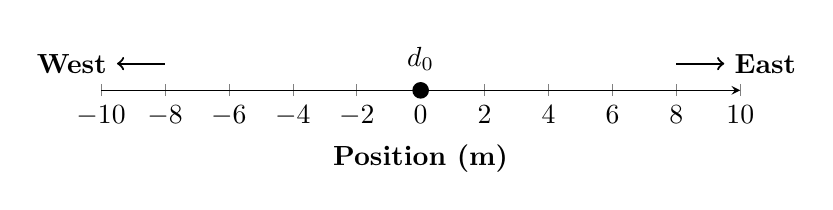
\begin{tikzpicture}
    \begin{axis}[
        width=0.8\textwidth,
        axis lines = left,
        axis y line=none,
        xlabel = \textbf{Position (m)},
        ymin=0, ymax=1, 
        xmin=-10, xmax=10,
        xtick={-10,-8,...,12},
        clip=false,
        ]
        \draw[->,thick] (axis cs: 8,0.05) -- (axis cs: 9.5,0.05) node[right] {\textbf{East}};
        \draw[->,thick] (axis cs: -8,0.05) -- (axis cs: -9.5,0.05) node[left] {\textbf{West}};
        \fill (axis cs: 0,0) circle[radius=3pt] node[above,inner sep=7pt] {$d_0$};
    \end{axis}
    \end{tikzpicture}
\end{figure}

\question \label{ques:cat_start}
What is the distance traveled?

\begin{solution}
\begin{equation*}
    16 + 7 + 3 = \SI{26}{m}
\end{equation*}
\end{solution}

\begin{choices}
\CorrectChoice 26 meters
\choice 12 meters
\choice 16 meters
\choice 10 meters
\end{choices}

\question
What is the magnitude of the displacement?

\begin{solution}
\begin{equation*}
  \mathrm{displacement} = 16 - 7 + 3 = \SI{12}{m \ East}  
\end{equation*}

Therefore, magnitude of displacement is 12 meters.
\end{solution}

\begin{choices}
\choice \SI{-12}{meters}
\choice 26 meters
\choice \SI{-26}{meters}
\CorrectChoice 12 meters
\end{choices}

\question \label{ques:cat_end}
What is the direction of the displacement?

\begin{solution}
East
\end{solution}

\begin{choices}
\CorrectChoice East
\choice West
\choice North
\choice South
\end{choices}

% \vspace{1em} \hrule

% \question
% If a space shuttle orbits Earth once, what is the shuttle’s distance traveled and displacement?

% \begin{choices}
% \choice Distance and displacement both are zero.
% \CorrectChoice Distance is circumference of the circular orbit. Displacement is zero.
% \choice Distance is zero. Displacement is circumference of the circular orbit.
% \choice Distance and displacement both are equal to circumference of the circular orbit.
% \end{choices}

% \begin{solution}
% The distance traveled is just the length of its circular orbit. Its displacement is 0 because the shuttle ended where it started.
% \end{solution}

% \begin{EnvUplevel}
% \textbf{Read the following prompt. Then answer Questions~\ref{ques:Skier_start} through~\ref{ques:Skier_end}.}

% A skier moves 53 meters eastward, then 71 meters westward, and finally 16 meters eastward. 
% \end{EnvUplevel}


% \question \label{ques:Skier_start}
% What is the distance traveled?

% \begin{choices}
% \choice 2 meters
% \choice 53 meters
% \choice 16 meters
% \CorrectChoice 140 meters
% \end{choices}

% \question
% What is the magnitude of the displacement?

% \begin{choices}
% \choice 140 meters
% \choice 71 meters
% \CorrectChoice 2 meters
% \choice Cannot be determined.
% \end{choices}

% \question \label{ques:Skier_end}
% What is the direction of the displacement?

% \begin{choices}
% \choice East
% \CorrectChoice West
% \choice North   
% \choice South
% \end{choices}

% \vspace{1em} \hrule

% \question
% If $x_0 = \SI{10}{m}$ and $x_f = \SI{3}{m}$, what is the displacement?

% \begin{solution}
% \begin{equation*}
%     \Delta{x} = x_f - x_0 = 3 - 10 = \SI{-7}{m} 
% \end{equation*}
% \end{solution}

% % \begin{choices}
% % \choice \SI{7}{m}
% % \CorrectChoice \SI{-7}{m} 
% % \choice \SI{13}{m}
% % \choice \SI{-13}{m}
% % \end{choices}

% \vspace{1em}
% \hrule

% \question
% Open ``The Moving Man'' simulation (\href{https://archive.cnx.org/specials/e2ca52af-8c6b-450e-ac2f-9300b38e8739/moving-man/}{click here}). 

% \begin{parts}
% \part When referring to the Man's position as $x = \SI{8}{m}$, what does the ``m'' mean?
% \begin{solution}
% The ``m'' stands for ``meters'' and is the SI unit of position ($x$).
% \end{solution}

% \part What is his displacement if he moves from the house to $x = \SI{4}{m}$?
% \part What is his displacement from the tree to $x = \SI{-3}{m}$?
% \part What is the displacement from the tree to the house?
% \end{parts}

% \vspace{1em}
% \hrule


% \begin{EnvUplevel}
% \textbf{Refer to the figure below and answer questions \ref{ques:bird_start} through \ref{ques:bird_end}.}
% \end{EnvUplevel}


% \begin{figure}[h!]
%     \centering
%     \begin{tikzpicture}
%     \begin{axis}[
%         width=0.8\textwidth,
%         axis lines = left,
%         axis y line=none,
%         xlabel = \textbf{Position (m)},
%         ymin=0, ymax=1, 
%         xmin=-10, xmax=10,
%         xtick={-10,-8,...,12},
%         clip=false,
%         ]
%         \node at (axis cs: -7.95,0.04)
%         {\includegraphics[scale=0.05]{Figures/tree.jpg}};
%         \node at (axis cs: 8,0.04)
%         {\includegraphics[scale=0.05]{Figures/house.png}};
%         \fill (axis cs: -5,0) circle[radius=3pt] node[above,inner sep=7pt] {\textbf{A}};
%         \fill (axis cs: -2,0) circle[radius=3pt] node[above,inner sep=7pt] {\textbf{B}};
%         \fill (axis cs: 0,0) circle[radius=3pt] node[above,inner sep=7pt] {\textbf{C}};
%         \fill (axis cs: 4,0) circle[radius=3pt] node[above,inner sep=7pt] {\textbf{D}};
%         \fill (axis cs: 7,0) circle[radius=3pt] node[above,inner sep=7pt] {\textbf{E}};
%     \end{axis}
%     \end{tikzpicture}
% \end{figure}

% \question \label{ques:bird_start}
% A bird moves from the \textbf{house} to \textbf{B}. What is the distance traveled?

% \begin{choices}
% \CorrectChoice 10 m
% \choice \SI{-10}{m}
% \choice 8 m
% \choice \SI{-2}{m}
% \end{choices}

% \begin{solution}
% 10 meters
% \end{solution}

% \question
% A bird moves from the \textbf{tree} to \textbf{C} to \textbf{A}. What is its displacement?

% \begin{choices}
% \CorrectChoice \SI{3}{m}
% \choice \SI{-5}{m}
% \choice \SI{13}{m}
% \choice \SI{-3}{m}
% \end{choices}

% \begin{solution}
% The initial and final positions are $x_0 = -8$ and $x_f = -5$.

% \begin{equation*}
% \Delta{x} = x_f - x_0 = -5 - (-8) = \SI{3}{m}   
% \end{equation*}
% \end{solution}

% \question
% A bird moves from \textbf{C} to \textbf{D} to \textbf{B}. What is the direction of its displacement?

% \begin{solution}
% negative ($-$)
% \end{solution}

% \begin{choices}
% \choice positive ($+$)
% \CorrectChoice negative ($-$)
% \choice south
% \choice north
% \end{choices}

% \question
% A bird moves from \textbf{E} to \textbf{D} to the \textbf{house}. What is the distance traveled?

% \begin{solution}
% 7 meters
% \end{solution}

% \begin{choices}
% \choice \SI{-1}{m}
% \choice 4 m
% \CorrectChoice 7 m
% \choice 3 m
% \end{choices}


% \question
% A bird moves from the \textbf{house} to the \textbf{tree} to \textbf{C} to the \textbf{tree} and to the \textbf{house}. What is its displacement?

% \begin{solution}
% zero
% \end{solution}

% \begin{choices}
% \CorrectChoice zero
% \choice \SI{48}{m}
% \choice \SI{-16}{m}
% \choice \SI{8}{m}
% \end{choices}


% \question \label{ques:bird_end} 
% The bird takes the following path: $\boldsymbol{\mathrm{house \rightarrow tree \rightarrow B \rightarrow C \rightarrow A \rightarrow D \rightarrow A}}$


% \begin{parts}
% \part What is the bird's displacement over the entire trip?
% \begin{solution}
% \SI{-13}{m}
% \end{solution}
% \part What total distance was travelled by the bird?
% \end{parts}


% % \begin{choices}
% % \choice \SI{47}{m}
% % \correctchoice \SI{-13}{m}
% % \choice \SI{-47}{m}
% % \choice \SI{13}{m}
% % \end{choices}


% \vspace{1em}
% \hrule

% \question
% If a biker rides west for 50 miles from his starting position, then turns and bikes back east 80 miles, what is his displacement?

% \begin{choices}
% \choice 130 miles
% \CorrectChoice 30 miles east
% \choice 30 miles west
% \choice Cannot be determined from the information given
% \end{choices}

% \begin{solution}
% If east is assumed to be the positive direction, the initial displacement will be $-50$ mi (west is negative), while the second displacement will be 80 mi. Adding the displacements: $-50 + 80 = 30$ mi east.
% \end{solution}

% \question
% A person travels 6 meters north, 4 meters east, and 6 meters south. What is the displacement?

% \begin{choices}
% \choice \SI{16}{\meter} east
% \choice \SI{6}{\meter} north
% \choice \SI{6}{\meter} south
% \CorrectChoice \SI{4}{\meter} east
% \end{choices}

% \question % Like Check Your Understanding 2.1 #5
% What is the difference between distance and displacement?

% \begin{solution}
% (\textit{Answers will vary.}) Distance is a vector (i.e., has magnitude but no direction), while displacement is a vector (i.e., has both magnitude and direction).
% \end{solution}

\clearpage
\section*{2.2 Speed and Velocity}
\subsection*{Speed}

\question
A pitcher throws a baseball from the pitcher's mound to home plate in \SI{0.46}{s}. The distance is \SI{18.4}{m}. What was the average speed of the baseball?

\begin{choices}
\correctchoice \SI{40.0}{m/s}
\choice \SI{72.9}{m/s}
\choice \SI{1.03}{m/s}
\choice \SI{8.54}{m/s}
\end{choices}

\begin{solution}
    $\text{distance} = \SI{18.4}{\meter}$, $\text{time}=\SI{0.46}{\second}$

\begin{equation*}
    \text{speed} = \frac{\text{distance}}{\text{time}} = \SI{40}{\meter/\second}
\end{equation*}
\end{solution}

\question
Four bicyclists travel different distances and times along a straight path. \\
Which cyclist traveled with the GREATEST average speed?

\begin{choices}
\choice Cyclist 1 travels \SI{95}{m} in \SI{27}{s}.
\choice Cyclist 2 travels \SI{87}{m} in \SI{22}{s}.
\choice Cyclist 3 travels \SI{106}{m} in \SI{26}{s}.
\CorrectChoice Cyclist 4 travels \SI{108}{m} in \SI{24}{s}.
\end{choices}

\begin{solution}
The average speed for cyclist 4 is found by dividing the distance (108 m) by the time (24 s) to give 4.5 m/s. Doing the same for the remaining cyclists results in a lower average speed for each.
\end{solution}


\question
A cart crosses a 228-cm track in 2.00 seconds. What was its average speed?

\begin{choices}
    \choice \SI{114}{m/s}
    \choice \SI{228}{m/s}
    \correctchoice \SI{1.14}{m/s}
    \choice \SI{2.28}{m/s}
\end{choices}

% \question
% Suppose you travel 12.5 km in 18.3 minutes. What is your average speed in kilometers per hour? (Note: Average speed is distance traveled divided by time of travel.)

% \begin{solution}
% \begin{equation*}
%     \mathrm{average\ speed = \frac{distance}{time}} = \frac{\SI{12.5}{\kilo\meter}}{\SI{18.3}{\minute}} = \SI[per-mode=fraction]{0.683}{\kilo\meter\per\minute}
% \end{equation*}

% \begin{equation*}
%     \SI[per-mode=fraction]{0.683}{\kilo\meter\per\minute} \times \frac{\SI{60}{\min}}{\SI{1}{\hour}} = \framebox{\SI{41.0}{\kilo\meter/\hour}}
% \end{equation*}
% \end{solution}

% \question
% An airplane travels 15 km in 5.0 minutes. What is its average speed in meters per second? (Note: Average speed is distance traveled divided by time of travel.)

% \begin{solution}
% \begin{equation*}
%     \mathrm{average\ speed = \frac{distance}{time}} = \frac{\SI{15}{\kilo\meter}}{\SI{5.0}{\minute}} = \SI[per-mode=fraction]{3.0}{\kilo\meter\per\minute}
% \end{equation*}

% \begin{equation*}
%     \SI[per-mode=fraction]{3.0}{\kilo\meter\per\minute} \times \frac{\SI{1}{\minute}}{\SI{60}{\second}} \times \frac{\SI{1000}{\meter}}{\SI{1}{\kilo\meter}} = \framebox{\SI{50}{\meter/\second}}\ .
% \end{equation*}
% \end{solution}


% \question
% A car travels 150 kilometers in 3.2 hours. What is the car's average speed?

% \begin{solution}
% The \textit{Known} quantities are

% \begin{itemize}
%     \item $\mathrm{distance} = \SI{150}{\km}$
%     \item $\mathrm{time} = \SI{3.2}{\hour}$
% \end{itemize}

% The average speed is

% \begin{equation*}
%     s_{\mathrm{avg}} = \mathrm{\frac{distance}{time}} = \SI[per-mode=symbol]{47}{\km\per\hour}\ .
% \end{equation*}
% \end{solution}

\question
A soccer ball travels with an average speed of \SI{16}{m/s} for \SI{2.5}{s}. How far did the ball travel?

\begin{choices}
    \choice \SI{6.4}{m}
    \choice \SI{0.15}{m}
    \choice \SI{16}{m}
    \correctchoice \SI{40}{m}
\end{choices}

\question
Imagine you and Usain Bolt have a race. Your average speeds are \SI{6.3}{m/s} and \SI{10.4}{m/s}, respectively. If you both run for 15 seconds, what distances will you and Bolt travel?

\begin{choices}
    \choice  \SI{0.42}{m};\ \ \SI{94.5}{m}
    \choice  \SI{156}{m};\ \ \SI{2.38}{m}
    \choice  \SI{2.38}{m};\ \ \SI{0.42}{m}
    \correctchoice \SI{94.5}{m};\ \ \SI{156}{m} 
\end{choices}

\question % Like Ch. 2 #18
You sit in an airplane that is moving at an average speed of 
\SI{900}{km/h} (\SI{0.25}{km/s}). During the \SI{8.0}{s}
that you glance out the window, how far has the plane traveled?

\begin{choices}
\CorrectChoice \SI{2.0}{km}
\choice \SI{7200}{km}
\choice \SI{113}{km}
\choice \SI{0.031}{km}
\end{choices}


\subsection*{Velocity}
\question % Like Ch. 2 Worked Example
A student has a displacement of 720 m north in 80 s. What was the student's average velocity?

\begin{choices}
\choice \SI{8.0}{m/s}
\CorrectChoice \SI{9.0}{m/s}
\choice \SI{7.6}{m/s}
\choice \SI{13}{m/s}
\end{choices}


\question
A student has a displacement of \SI{739}{m} north in \SI{162}{s}. What was the student's average velocity?

\begin{solution}
    The given quantities are $\Delta{x} = \SI{739}{m}$ and $\Delta{t} = \SI{162}{s}$. Average velocity is

\begin{equation*}
        \bar{v} = \frac{\Delta{x}}{\Delta{t}} = \SI{4.56}{m/s\ north}
\end{equation*}
\end{solution}



\question % Like Ch. 2 Worked Example
Layla jogs with an average velocity of 6.1 m/s east. What is her displacement after 75 seconds?

\begin{choices}
\choice 0.081 m
\choice 12.3 m
\CorrectChoice 458 m
\choice 6.1 m
\end{choices}


\question % Like High-School Physics Ch. 2 Worked Example
Phillip walks along a straight path from his house to his school. How long will it take him to get to school if he walks \SI{540}{m} west with an average velocity of 1.5 m/s west?

\begin{choices}
\CorrectChoice \SI{6.0}{min}
\choice \SI{360}{min}
\choice \SI{5.4}{min}
\choice \SI{810}{min}


\end{choices}

\question
In the definition of velocity, what physical quantity is changing over time?

\begin{choices}
\choice speed
\choice distance
\choice acceleration
\CorrectChoice position vector
\end{choices}

\begin{solution}
A velocity vector gives the rate of change of the position vector.
\end{solution}

\question
Yes or no---Is it possible to determine a car’s instantaneous velocity from just the speedometer reading?

\begin{choices}
\CorrectChoice No, it reflects speed but not the direction.
\choice No, it reflects the average speed of the car.
\choice Yes, it sometimes reflects instantaneous velocity of the car.
\choice Yes, it always reflects the instantaneous velocity of the car.
\end{choices}

\question
A car travels with an average speed of 23 m/s for 82 s. Which of the following could NOT have been the car's displacement?

\begin{choices}
\choice 1,700 m east
\CorrectChoice 1,900 m west
\choice 1,600 m north
\choice 1,500 m south
\end{choices}

\begin{solution}
If the car moved in a straight line, its displacement would be $(23\ \mathrm{m/s})(82\ \mathrm{s}) = 1,886\ \mathrm{m}$. Any other path would result in a displacement of smaller magnitude. So, 1,900 m west is not possible.
\end{solution}

\question 
A car is moving on a straight road at a constant speed in a single direction. Which of the following statements is true?

\begin{choices}
\choice Average velocity is zero.
\CorrectChoice The magnitude of average velocity is equal to the average speed.
\choice The magnitude of average velocity is greater than the average speed.
\choice The magnitude of average velocity is less than the average speed.
\end{choices}

\begin{solution}
The magnitude of its velocity will be equal to the speed if the direction of motion is not changing.
\end{solution}


\question
A student has a displacement of 304 m north in 180 s. What was the student's average velocity?

\begin{solution}
The known quantities are:

\begin{itemize}
    \item displacement: $\Delta{x} = \SI{304}{\meter}$
    \item change in time: $\Delta{t} = \SI{180}{\second}$
\end{itemize}

The average velocity is

\begin{equation*}
    v_{\mathrm{avg}} = \frac{\Delta{x}}{\Delta{t}} = \frac{\SI{304}{\meter}}{\SI{180}{\second}} = \SI[per-mode=symbol]{1.7}{\meter\per\second\ north}
\end{equation*}
\end{solution}



\question
Cassie walked to her friend’s house with an average speed of 1.40 m/s. The distance between the houses is 205 m. How long did the trip take her?

\begin{solution}
    $\text{speed} = \SI{1.40}{\meter/\second}$, $D = \SI{205}{\meter/\second}$

\begin{equation*}
    \text{time} = \frac{\text{distance}}{\text{speed}} = \SI{146}{\second}
\end{equation*}
\end{solution}

\question
What is the distance traveled by an object that moves with an average speed of 6.0 meters per second for 8.0 seconds?

\begin{solution}
    $\text{speed} = \SI{6.0}{\meter/\second}$, $\text{time} = \SI{8.0}{\second}$

\begin{equation*}
    \text{distance} = \text{speed} \times \text{time} = \SI{48}{\meter} 
\end{equation*}
\end{solution}


\question
A train on a track makes a trip from the 5.25-km mark to the 3.75-km mark. What is the average velocity (in km/h) if the trip takes 5.0 min?

\begin{solution}
    \textbf{Answer}: $\SI{-18.0}{km/h}$. See \textit{OpenStax}: Example 2.6 (\href{https://openstax.org/books/college-physics/pages/2-4-acceleration}{link})
\end{solution}

\question
Layla jogs with an average velocity of 2.4 m/s east. What is her displacement after 46 s?

\begin{solution}
    $v = \SI{2.4}{m/s\ east}$, $t = \SI{46}{s}$

\begin{equation*}
    \Delta{x} = v \cdot t = \SI{110}{m\ east}
\end{equation*}
\end{solution}


\question
How long will it take Phillip to get to school if he walks 428 m west with an average velocity of 1.70 m/s west?

\begin{solution}
    $\Delta{x} = \SI{428}{m\ west}$, $v = \SI{1.70}{m/s\ west}$

\begin{equation*}
    t = \frac{\Delta{x}}{v} = \SI{252}{s}
\end{equation*}
\end{solution}


\section*{2.3 Position vs.~Time Graphs}

\question
Which of the following information about motion can be determined by looking at a position vs.~time graph that is a straight line?

\begin{choices}
\choice frame of reference
\choice average acceleration
\CorrectChoice velocity
\choice direction of force applied
\end{choices}

\question
What is the slope of a straight line graph of position vs.~time?

\begin{choices}
\CorrectChoice Velocity
\choice Displacement
\choice Distance
\choice Acceleration
\end{choices}

\begin{solution}
The slope of the line is the rise (position) over the run (time). ``Position over time'' units are for velocity.
\end{solution}


\question
True or False: The position vs.~time graph of an object that is speeding up is a straight line.

\begin{choices}
\choice True
\CorrectChoice False
\end{choices}



\begin{EnvUplevel}
\textbf{Refer to Figure~\ref{fig:Ch2_Prob6} and answer Questions \ref{ques:start} through \ref{ques:Ch2_Prob35}.}
\end{EnvUplevel}



\begin{EnvUplevel}
\textbf{Refer to the figure below and answer questions \ref{ques:runner_start} though \ref{ques:runner_end}.}

The graph below represents the motion of a runner.
\end{EnvUplevel}

\begin{figure}[h!]
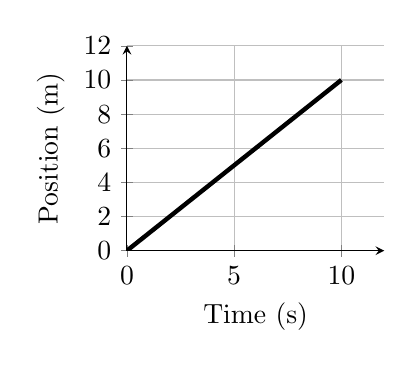
\begin{tikzpicture}
\begin{axis}[width=0.4\textwidth,
    axis y line=left, 
    axis x line=left,
    ymin=0, ymax=12,
    xmin=0, xmax=12,
    ylabel = Position (m),
    xlabel = Time (s),
    grid = both,
    ytick={0,2,...,12}
]
\addplot[
    %color=green!67!black,
    color=black,
    mark options={color=black},mark=none,
    ultra thick,
    ]
    coordinates {
    (0,0)
    (10,10)
    };
\end{axis}
\end{tikzpicture}
\end{figure}

\question \label{ques:runner_start} 
In the space to the right of the \textbf{position vs.~time} graph, draw the corresponding \textbf{velocity vs.~time} graph. Label the velocity and time axis, including units. Label the numbers on the axes. 

\begin{solution}

\begin{tikzpicture}
\begin{axis}[color=black,axis y line=left, 
    axis x line=left,
    ymin=0, ymax=2,
    xmin=0, xmax=10,
    ylabel = Velocity (m/s),
    xlabel = Time (s),
    grid = none,
    ytick={0,1,2}
]
\addplot[
    %color=green!67!black,
    color=black,
    mark options={color=black},mark=none,
    ultra thick,
    ]
    coordinates {
    (0,1)(10,1)
    };
\end{axis}
\end{tikzpicture}
\end{solution}


\question 
What is the \textbf{displacement} during the entire time interval?

\begin{solution}
From the \textbf{position vs.~time graph}, the initial and final positions are $x_0=0$ and $x_f = \SI{10}{m}$. Displacement is

\begin{equation*}
    \Delta{x} = x_f - x_0 = \SI{10}{m}.
\end{equation*}
\end{solution}

\question \label{ques:runner_end} 
What is the \textbf{average velocity} during the entire time interval?

\begin{solution}
For a \textbf{position vs.~time graph} that is linear, \textbf{average velocity} is the slope of the line. Choosing any two coordinates $(t_0,x_0)$ and $(t_f,x_f)$ yields

\begin{equation*}
    v = \frac{\Delta{x}}{\Delta{t}} = \frac{x_f - x_0}{t_f - t_0} = \SI{1.0}{m/s}
\end{equation*}
\end{solution}





\vspace{1em} \hrule

\question
The data in the table shows the measured distance that a train travels from its station versus time. Use the coordinate system to plot the line graph of the data.

\begin{minipage}{0.4\textwidth}
\begin{tabular}{l|l}
    \textbf{Time (min)} & \textbf{Distance (km)} \\
    \hline\hline
    0 & 0\\
    10 & 24\\
    20 & 36\\
    30 & 60\\
    40 & 84\\
    50 & 97\\
    60 & 116\\
    70 & 140\\
\end{tabular}
\end{minipage}\hfill
\begin{minipage}{0.6\textwidth}
\centering
\scalebox{1}{
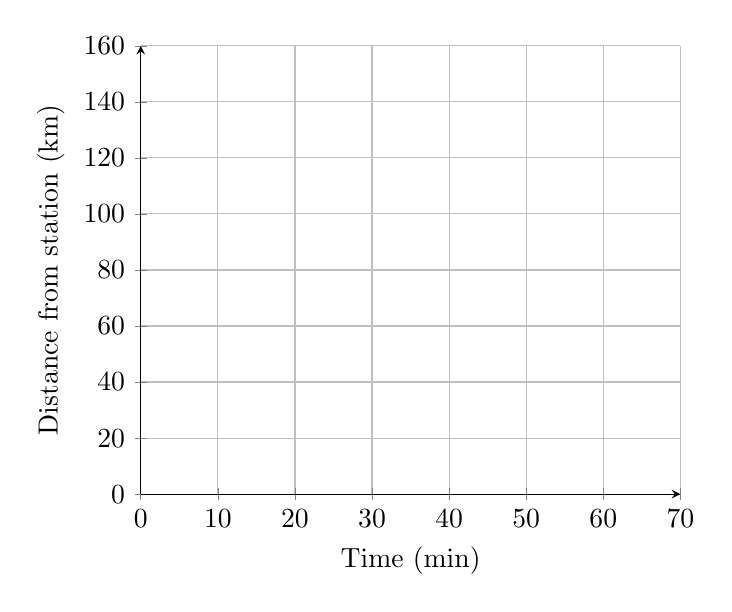
\begin{tikzpicture}
\begin{axis}[axis y line=left, 
    axis x line=left,
    ymin=0, ymax=160,
    xmin=0, xmax=70,
    ylabel = Distance from station (km),
    xlabel = Time (min),
    grid=both,
    ytick={0,20,...,160}
]
\addplot[
    %color=green!67!black,
    color=black,
    mark options={color=black},mark=*,
    ultra thick,
    ]
    coordinates {
    %(0,0)(10,24)(20,36)(30,60)(40,84)(50,97)(60,116)(70,140)
    };
\end{axis}
\end{tikzpicture}
}
\end{minipage}

\section*{2.4 Velocity vs.~Time Graphs}

\subsection*{Graphing Velocity as a Function of Time}

\question
What does the area under a velocity vs.~time graph line represent?

\begin{choices}
\choice Acceleration
\CorrectChoice Displacement
\choice Distance
\choice Instantaneous velocity
\end{choices}

\begin{EnvUplevel}
\textbf{For questions \ref{ques:Unit02_Elevator1} and \ref{ques:Unit02_Elevator2}, refer to the velocity vs.~time graph shown in Figure~\ref{fig:Unit02_Fig2.20}.}
\end{EnvUplevel}

\begin{figure}[h!]
    \centering
    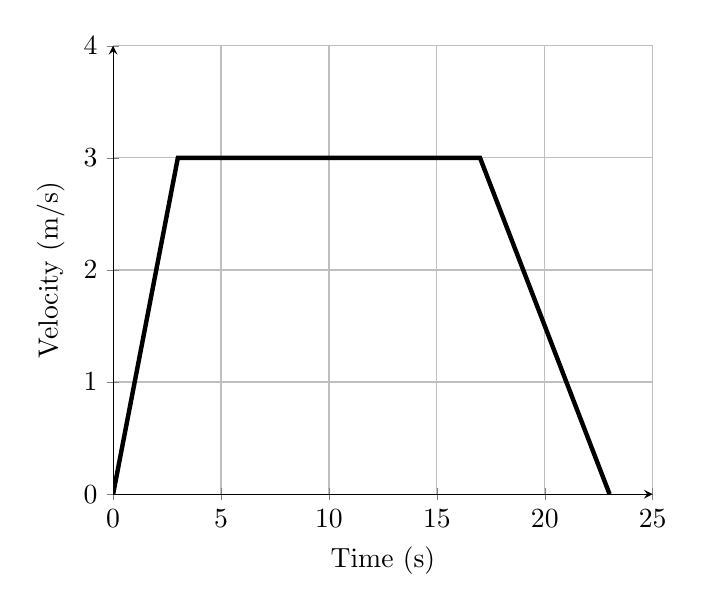
\begin{tikzpicture}
    \begin{axis}[axis y line=left, 
        axis x line=left,
        ymin=0, ymax=4,
        xmin=0, xmax=25,
        ylabel = Velocity (m/s),
        xlabel = Time (s),
        grid=both,
        ytick={0,1,...,4}
    ]
    \addplot[
        %color=green!67!black,
        color=black,
        %mark options={color=black},mark=*,
        ultra thick,
        ]
        coordinates {
        (0,0)(3,3)(17,3)(23,0)
        };
    \end{axis}
    \end{tikzpicture}
    \caption{A $v$ vs.~$t$ graph of an elevator moving up some floors. Suppose the elevator is initially at rest. It then speeds up for 3 seconds, maintains that velocity for 15 seconds, then slows down for 5 seconds until it stops.}
    \label{fig:Unit02_Fig2.20}
\end{figure}

\question \label{ques:Unit02_Elevator1}

The instantaneous velocity at t = 10 s is \underline{\hspace{2cm}}. The instantaneous velocity at t = 23 s is \underline{\hspace{2cm}}.

\begin{choices}
\choice \SI[per-mode=symbol]{0.0}{\meter\per\second}; \SI[per-mode=symbol]{0.0}{\meter\per\second}
\choice \SI[per-mode=symbol]{0.0}{\meter\per\second}; \SI[per-mode=symbol]{3.0}{\meter\per\second}
\CorrectChoice \SI[per-mode=symbol]{3.0}{\meter\per\second}; \SI[per-mode=symbol]{0.0}{\meter\per\second}
\choice \SI[per-mode=symbol]{3.0}{\meter\per\second}; \SI[per-mode=symbol]{1.5}{\meter\per\second}
\end{choices}

\question \label{ques:Unit02_Elevator2}

Calculate the net displacement and the average velocity of the elevator over the time interval shown.

\begin{choices}
\choice Net displacement is 45 m and average velocity is 2.10 m/s.
\choice Net displacement is 45 m and average velocity is 2.28 m/s.
\choice Net displacement is 57 m and average velocity is 2.66 m/s.
\CorrectChoice Net displacement is 57 m and average velocity is 2.48 m/s.
\end{choices}





\end{questions}
\end{document}

\textbf{OTHER QUESTIONS}



% % \section*{Distance vs.~Displacement}

% % \hrule



% \vspace{1em} \hrule


% % \begin{EnvUplevel}
% % Suppose you take a trip from Houston to San Antonio to Austin.
% % \end{EnvUplevel}

% % \begin{figure}[h!]
% %     \centering
% %     \includegraphics[width=0.7\textwidth]{Figures/Unit02_Fig_Texas.png}
% %     \caption{A map of Texas.}
% %     \label{fig:Unit02_Fig_Texas}
% % \end{figure}

% % \question
% % Draw the total distance you travel.

% % \question
% % Draw your displacement vector.

% % \vspace{1em} \hrule



% % \begin{EnvUplevel}
% % For questions \ref{ques:BusRoute1} and~\ref{ques:BusRoute2}, refer to Figure~\ref{fig:Unit02_Fig_BusRoute}.
% % \end{EnvUplevel}

% % \begin{figure}[h!]
% %     \centering
% %     \includegraphics[width=0.5\textwidth]{Figures/Unit02_Fig_BusRoute.png}
% %     \caption{The route of a school bus showing the initial and final positions.}
% %     \label{fig:Unit02_Fig_BusRoute}
% % \end{figure}

% % \question \label{ques:BusRoute1}
% % What is the magnitude of the total displacement of the bus?

% % \begin{choices}
% % \choice 400 m
% % \choice 500 m
% % \CorrectChoice 800 m
% % \choice 1800 m
% % \end{choices}

% % \question \label{ques:BusRoute2}
% % What is the total distance traveled by the bus?

% % \begin{choices}
% % \choice 400 m
% % \choice 500 m
% % \choice 800 m
% % \CorrectChoice 1800 m
% % \end{choices}

% % \question
% % A student on her way to school walks four blocks east, three blocks north, and another four blocks east, as shown below. 

% % \begin{figure}[h!]
% %     \centering
% %     \includegraphics[width=0.7\textwidth]{Figures/Unit02_Fig_SchoolRoute.png}
% %     \caption{The route from home to school.}
% %     \label{fig:Unit02_Fig_SchoolRoute}
% % \end{figure}

% % Compared to the distance she walks, the magnitude of her displacement from home to school is

% % \begin{choices}
% % \CorrectChoice less
% % \choice greater
% % \choice the same
% % \end{choices}





% \section*{Speed}



% \section*{Velocity}





% \section*{Graphing Position as a Function of Time}



% % \begin{EnvUplevel}
% % Figure~\ref{fig:Unit02_Fig2.10} may be useful for the following questions.
% % \end{EnvUplevel}

% % \begin{figure}[h!]
% %     \centering
% %     \includegraphics[width=3in]{Figures/Unit02_Fig2.10.jpg}
% %     \caption{The diagram shows a straight-line graph. The equation for the straight line is $y$ equals $mx + b$.}
% %     \label{fig:Unit02_Fig2.10}
% % \end{figure}



% % \question
% % What is the runner’s net displacement over the time shown?

% % \vspace{0.5em}

% % \begin{minipage}{0.2\textwidth}
% % \begin{choices}
% % \choice \SI{6}{\m}
% % \CorrectChoice \SI{4}{\m}
% % \choice \SI{10}{\m}
% % \choice \SI{12}{\m}
% % \end{choices}
% % \end{minipage}%
% % \begin{minipage}{0.7\textwidth}
% % \centering
% % \begin{tikzpicture}
% % \begin{axis}[axis y line=left, 
% %     axis x line=left,
% %     ymin=0, ymax=14,
% %     xmin=0, xmax=12,
% %     ylabel = Position (m),
% %     xlabel = Time (s),
% %     grid=both,
% %     ytick={0,2,...,14}
% % ]
% % \addplot[
% %     %color=green!67!black,
% %     color=black,
% %     %mark options={color=black},mark=*,
% %     ultra thick,
% %     ]
% %     coordinates {
% %     (0,0)(2,6)(4,6)(6,12)(8,4)(10,4)
% %     };
% % \end{axis}
% % \end{tikzpicture}
% % \end{minipage}

% % \question
% % What is the runner’s net displacement over the time shown?

% % \vspace{0.5em}

% % \begin{minipage}{0.2\textwidth}
% % \begin{choices}
% % \CorrectChoice \SI{0}{\m}
% % \choice \SI{8}{\m}
% % \choice \SI{6}{\m}
% % \choice \SI{14}{\m}
% % \end{choices}
% % \end{minipage}%
% % \begin{minipage}{0.7\textwidth}
% % \centering
% % \begin{tikzpicture}
% % \begin{axis}[axis y line=left, 
% %     axis x line=left,
% %     ymin=0, ymax=14,
% %     xmin=0, xmax=12,
% %     ylabel = Position (m),
% %     xlabel = Time (s),
% %     grid=both,
% %     ytick={0,2,...,14}
% % ]
% % \addplot[
% %     %color=green!67!black,
% %     color=black,
% %     %mark options={color=black},mark=*,
% %     ultra thick,
% %     ]
% %     coordinates {
% %     (0,0)(2,8)(4,8)(6,0)(8,6)(10,0)
% %     };
% % \end{axis}
% % \end{tikzpicture}
% % \end{minipage}



% % \question In algebra, the equation of a straight line is $y = mx + b$. What is the equivalent equation of a straight line on a position vs.~time graph? Express the equation in terms of $d$, $t$, $d_0$, and $v$.

% % \question
% % Consider the one-way trip from home to school, as shown in Figure~\ref{fig:Unit02_Fig_PositionVsTime1} below.

% % \begin{parts}
% % \part What physical quantity does $d_0$ represent?
% % \part What is the numerical value of $d_0$?
% % \part In the linear equation $y = mx + b$, what does $m$ mean?
% % \part If a position vs.~time graph that is a straight line is model by $y = mx + b$, which variable represents $d_0$?
% % \part In a linear graph, slope is \textit{rise} over \textit{run} (see Figure~\ref{fig:Unit02_Fig2.10}). In a position vs.~time graph, the \textit{rise} is the \textit{change in} \underline{\hspace{2cm}} and the \textit{run} is the \textit{change in} \underline{\hspace{2cm}}.
% % \part Which symbol represents \textit{change in}?
% % \part Use the variables that represent \textbf{position}, \textbf{time}, and the \textit{change in} these to express \textit{rise} over \textit{run}. \label{part:slope}
% % \part The fraction from Part~(\ref{part:slope}) represents the physical quantity \underline{\hspace{2cm}}. Therefore, the slope in a position vs.~time graph represents the \underline{\hspace{2cm}}.
% % \end{parts}

% % \begin{figure}[h!]
% %     \begin{minipage}{0.5\textwidth}
% %     \centering
% %     \includegraphics[width=3in]{Figures/Unit02_Fig2.4.jpg}
% %     \end{minipage}\hfill
% %     \begin{minipage}{0.5\textwidth}
% %     \centering
% %     \includegraphics[width=3in]{Figures/Unit02_Fig2.11.jpg}
% %     \end{minipage}
% %     \caption{Position vs.~time graph of a trip from home to school.}
% %     \label{fig:Unit02_Fig_PositionVsTime1}
% % \end{figure}



% \question
% Using the graph, what is the runner’s velocity from 4 to 10 s?

% \begin{figure}[h!]
%     \centering
%     \includegraphics{Unit2_Fig_TestPrep35.jpg}
%     \caption{}
%     \label{fig:Unit2_Fig_TestPrep35}
% \end{figure}

% \begin{choices}
% \choice $-3$ m/s
% \CorrectChoice $0$ m/s
% \choice $1.2$ m/s
% \choice $3$ m/s
% \end{choices}

% \begin{solution}
% Since the runner’s position is not changing from 4 s to 10 s, the runner’s velocity must be 0 m/s.
% \end{solution}


% \question
% Calculate the average velocity of the object shown in Figure~\ref{fig:Unit02_Fig_Ch2_PracProb15} over the whole time interval.

% \begin{figure}[h!]
%     \centering
%     \includegraphics[width=3in]{Figures/Unit02_Fig_Ch2_PracProb15.jpg}
%     \caption{A graph of $d$ vs.~$t$ for a moving object.}
%     \label{fig:Unit02_Fig_Ch2_PracProb15}
% \end{figure}

% \begin{choices}
% \CorrectChoice \SI[per-mode=symbol]{0.25}{\meter\per\second}
% \choice \SI[per-mode=symbol]{0.31}{\meter\per\second}
% \choice \SI[per-mode=symbol]{3.2}{\meter\per\second}
% \choice \SI[per-mode=symbol]{4.00}{\meter\per\second}
% \end{choices}

% \question
% How would you use a position vs.~time graph to construct a velocity vs.~time graph and vice versa?

% \underline{\hspace{2cm}} of position vs.~time curve is used to construct velocity vs.~time curve, and \underline{\hspace{2cm}} of velocity vs.~time curve is used to construct position vs.~time curve.

% \begin{choices}
% \choice Slope; slope
% \CorrectChoice Slope; area
% \choice Area; slope
% \choice Area; area
% \end{choices}

% \question
% Which statement best describes the relationship between instantaneous velocity and instantaneous speed?

% \begin{choices}
% \choice Instantaneous speed and instantaneous velocity are the same, even when there is a change in direction.
% \choice Instantaneous speed and instantaneous velocity cannot be the same even if there is no change in direction.
% \CorrectChoice Magnitude of instantaneous velocity is equal to instantaneous speed.
% \choice Magnitude of instantaneous velocity is always greater than instantaneous speed.
% \end{choices}

% \begin{solution}
% The instantaneous speed and the magnitude of the instantaneous velocity are the same.
% \end{solution}

% \question
% The following is a position vs.~time graph. Predict what the object's prediction will be at a later time.



% \question
% A graph of velocity vs. time of a ship coming into a harbor is shown.

% \begin{center}
% \begin{tikzpicture}
% \begin{axis}[width=3.5in,
%     axis y line=left, 
%     axis x line=left,
%     ymin=0, ymax=10,
%     xmin=0, xmax=10,
%     ylabel = {\Large $v$},
%     xlabel = {\Large $t$},
%     ytick={0,1,...,14},
%     yticklabels={,,},
%     xticklabels={,,},
%     ytick style={draw=none},
%     xtick style={draw=none},
%     ylabel style={rotate=-90},
% ]
% \addplot[
%     %color=green!67!black,
%     color=black,
%     mark options={color=black},mark=none,
%     ultra thick,
%     ]
%     coordinates {
%     (0,8)(2,8)(4,3)(9,0)
%     };
% \end{axis}
% \end{tikzpicture}
% \end{center}

% How would you describe the acceleration of the ship based on the graph?

% \begin{choices}
% \choice The ship is moving in the forward direction at a steady rate. Then it accelerates in the forward direction and then decelerates.
% \choice The ship is moving in the forward direction at a steady rate. Then it turns around and starts decelerating, while traveling in the reverse direction. It then accelerates, but slowly.
% \choice The ship is moving in the forward direction at a steady rate. Then it decelerates in the forward direction, and then continues to slow down in the forward direction, but with more deceleration.
% \CorrectChoice The ship is moving in the forward direction at a steady rate. Then it decelerates in the forward direction, and then continues to slow down in the forward direction, but with less deceleration.
% \end{choices}

% \section*{Defining Motion}

% \question
% Passenger A sits inside a moving train and throws a ball vertically upward. How would the motion of the ball be described by a fellow train passenger B and an observer C who is standing on the platform outside the train?

% \begin{choices}
% \CorrectChoice Passenger B sees that the ball has vertical, but no horizontal, motion. Observer C sees the ball has vertical as well as horizontal motion.
% \choice Passenger B sees the ball has vertical as well as horizontal motion. Observer C sees the ball has the vertical, but no horizontal, motion.
% \choice Passenger B sees the ball has horizontal, but no vertical, motion. Observer C sees the ball has vertical as well as horizontal motion.
% \choice Passenger B sees the ball has vertical as well as horizontal motion. Observer C sees the ball has horizontal, but no vertical, motion.
% \end{choices}


% \begin{choices}
% \choice Distance has both magnitude and direction, while displacement has magnitude but no direction.
% \CorrectChoice Distance has magnitude but no direction, while displacement has both magnitude and direction.
% \choice Distance has magnitude but no direction, while displacement has only direction.
% \choice There is no difference. Both distance and displacement have magnitude and direction.
% \end{choices}

% \question \label{ques:Ch2_Prob6} % Like Ch. 2 #6
% How are average velocity for only the first eight seconds and instantaneous velocity related? What is the runner's net displacement over the time shown?

% \begin{choices}
% \choice The net displacement is 8 m and the average velocity is two times the instantaneous velocity.
% \choice The net displacement is $8 + 12 = 20$ m and the average velocity is equal to the instantaneous velocity.
% \choice The net displacement is $8 + 12 = 20$ m and the average velocity is two times the instantaneous velocity.
% \CorrectChoice The net displacement is 8 m and the average velocity is equal to the instantaneous velocity.
% \end{choices}